\lhead{\emph{Related work}}
\chapter{Related work}
In this chapter specific research areas and systems related to this thesis are presented. First the current situation on mobile music player user interfaces is described. Then a wider description of two research areas; mobile HCI and multimodal interaction are presented before going into details about how previous developed interaction techniques within these two areas can be combined with a mobile music player UI. A graphical overview is shown in fig. \ref{fig:venn}.

\begin{figure}[htbp]
	\centering
		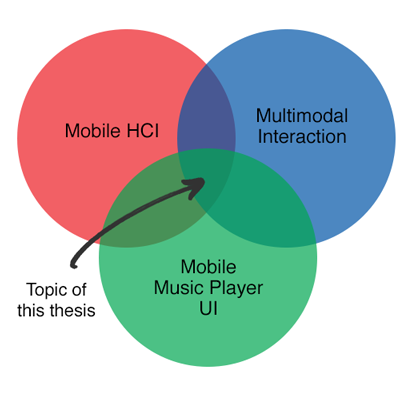
\includegraphics[width=0.5\textwidth,height=\textheight,keepaspectratio]{./Figures/venn.png}
		\rule{35em}{0.5pt}
	\caption[Venn diagram]{Thesis topic position}
	\label{fig:venn}
\end{figure}


\section{Mobile Music Player UI}

% intro
The rise of the smartphone and the introduction of music streaming services e.g. Spotify, Deezer, Pandora, WIMP and more have resulted in an increase in mobile music listening - in fact the number of mobile music listeners has more than doubled from 2011 to 2013 according to a study in America \cite{emarketer_music_2014}. Although mobile audio players have developed since the first portable cassette player by Sony in 1979 towards todays digital audio players with storage capacity e.g. smartphones, there is still a factor that remains - the way in which we interact with the device. E.g. like we needed the hands and eyes for rewinding or turning the tape on a cassette player, we need them as well for swiping to the preferred track in todays "typical" smartphone music application.

% typical interfaces, challenges
Todays "typical" Music Player UI could cause interaction challenges when a user is on the move. Imagine a biking scenario where the user wants to change music track in a smartphone music application. This would require: Fetching the device e.g. from a pocket, switching the screen on, maybe unlocking the screen with a password, navigating through the music application GUI, switch the screen of, put smartphone back in pocket. Also the smartphone touch interface requires bare fingers for input recognition so removing gloves (in winter season) could also be a step in the process. A process that happens while the user is navigating through traffic. Studies show that while a user is doing an activity a vital factor is to minimize the amount of distraction for interaction modes \cite{pascoe_using_2000}.

\subsection{Alternative Music Player UI's}
\label{sec:alternativemusicuis}
There exists music player interfaces that tries to avoid the before mentioned process when listening to music on the go.

% headset controller
Headset music controllers are physical buttons attached to the wire between headset and device. This controller typically includes play, stop, next track, previous track and volume buttons. Such a controller would require only one hand from the user to interact with a music application. This kind of interaction though assumes the user has created a playlist and knows in which order the tracks follows to navigate efficiently to the wanted track. Also this kind of interaction menu is 1-dimensional in the sense that numbers have to be placed in a sequence missing the opportunity to go into a submenu e.g. an album of an artist. It should also be taken into account that although only using one hand for interaction this could still create challenges e.g. when steering or hitting the breakes while biking could require both hands on the steering.

% voice recognition
Voice recognition could also be used for navigating a music application \cite{stewart_boling_voice_2013}. In this application example the user could request simple commands like play, stop, next/previous track and queue. Voice recognition however introduces accuracy and stability challenges especially in mobile noisy environments. At the same time speech commands are limited - it would introduce even more complexity if the system should be able to interpret detailed commands e.g. an artist name or even a track title.

% other alternatives
Other more alternative music player interaction modes also exists using motion sensors. A system that use foot gestures for changing music track has been developed and shows a highly efficient way of interacting while running \cite{smus_running_2010}. Another system also using gesture recognition controls a music player by placing a device on different body parts e.g. placing it by side of the head while nodding changes the music track \cite{strachan_bodyspace_2007}. 

All these systems have in common that they avoid the users visual attention but they are all limited to basic controls such as play, stop, next/previous track, volume up/down.


\section{Mobile Human Computer Interaction}
The term "Human Computer Interaction" involves the study, planning and design of the interaction between human and computers \cite{card_psychology_1983}. This term supports a view both from the computer and from the human perspective. From a computer perspective in the mobile HCI community challenges like short battery life, network volatility, limited memory/processing power typically arise and specific system design patterns have been designed to handle this \cite{roth_patterns_2002}. From a mobile human perspective the term "nomadic computing" can be used where the main requirements for such a system is defined as providing capabilities and services to the nomad as he/she moves from place to place in a transparent, integrated and convenient way \cite{sawhney_nomadic_2000}.

% this project
In this project a mobile music player for cyclists is developed so the focus will be on the interaction between a user and device while the user is in motion. This kind of interaction has also been defined as "interaction in motion" \cite{marshall_mobile_2013}.

\subsection{Interaction in motion}
\label{sec:interactioninmotion}
According to Marshall and Tennent \cite{marshall_mobile_2013} mobile interaction does not exist as most mobile systems are designed for active interaction when a user is standing still dedicating his/her full attention to the device. Specific mobile systems should instead allow the user to interact while in motion e.g. driving, running or in this thesis case biking. To develop such kind of system specific challenges needs to be solved and Marshall and Tennent have classified these into four categories \cite{marshall_mobile_2013}:

\begin{description}
\item[Cognitive Load]
Essentially this concept is decribed as a person only being able to pay attention to a certain amount of things at once. When this limit is reached the person stops paying attention to other things. This means that even though a person is able physically to sense, hear or feel multiple interaction tasks, it may not be possible to attend to all these tasks at the same time.

% from the systems point of view
Depending on the mobile interactive system this cognitive load can change over time. If a person is forced to actively attend or respond to the system the cognitive load is increased while a passive output from the system can decrease the cogntitive load. Also the content of information being addressed to the person can affect the cognitive load e.g. when making phone calls a discussion with an interviewer is less distracting than performing a simple memory test \cite{nunes_cognitive_2002}.

% environment
The cognitive load can also depend on environmental factors e.g. the movement activity in which the user is performing. Physical challenges e.g. walking a plane ground vs. climbing stairs can effect the mental demand of the user i.e. increase the cognitive load.

\item[Physical Constraints]
Mobile systems and user movement activities can both add constraints on the body position which could lead to a conflict making it hard or even impossible to interact. E.g. as mentioned earlier biking physically needs the hands for steering and eyes on the road while both of these body parts are used in the traditional smartphone interaction form (eyes on the screen, hands for touch gestures). This has been identified to be a major barrier to the use of mobile system whilst moving \cite{pielot_pocketmenu:_2012}.

\item[Terrain]
The terrain is described by the enviroment around a person while moving and interacting. Studies have shown that while running and interacting the terrain over which a person was running made a big difference in the interaction experience and the ability to concentrate on the output of the system \cite{marshall_using_2011}.

Physical terrain can be dynamic i.e. it can change over time while moving around different environments e.g. road obsticles, traffic, light level, rain, sound, etc. This could not only affect the user interaction experience but also the electronic device e.g. water or extreme cold/heat.

\item[Other people]
This class relates to other people during a interaction. For example in a crowded place the user needs to take care of people passing by while interacting with the mobile device. Or When biking the user needs to take care of people making an overhaul, communicating or waving back to a friend on the sidewalk. The social aspect of the environment a person is in can also have an impact on the device interaction e.g. in a quiet place a person would probably not use speech commands to interact with a device as this would be socially impolite.
\end{description}


\section{Multimodal interaction}
While the previous section was about planning and designing the interaction between humans and computers, this section describes how the actual information between a human and computer could be exchanged. 

\subsection{Modality definition and use}
Bolt was one of the first to define the term modality in a study where speech and gesture in combination was used as input to a system \cite{bolt_put-that-there:_1980}. Modalities has something to do with the mode of communication according to the human senses and input devices activated by humans \cite{jaimes_multimodal_2007,tzovaras_dimitrios_multimodal_2008}. The human senses are \textit{sight}, \textit{touch}, \textit{hearing}, \textit{smell} and \textit{taste}. Input modalities of many computer input devices can then be considered to correspond to these senses e.g. cameras (\textit{sight}), haptic sensors (\textit{touch}), microphones (\textit{hearing}). While the term multimodal has been used in many different contexts and disciplines this thesis will focus on Tzovaras definition: \textit{"During interaction, the user produces input modalities to the system and the system produces output modalities to the user. A multimodal interactive system is a system that uses at least two different modalities for input and/or output. And a unimodal system is a system which uses the same single modality for input and output"} \cite{tzovaras_dimitrios_multimodal_2008}. The word input is defined by \cite{jaimes_multimodal_2007} to be of great importance as in practice most interactions take place using multiple modalities e.g. typing a keyboard (\textit{touch}) while looking at the keys or screen (\textit{sight}) to see whats being typed.

% modality combinations
Modalities can be used in combination with each other in different ways. In the "Put that there" system \cite{bolt_put-that-there:_1980} modalities are used in a complementary combination as the user can point the items on a large display and select or move them by vocal commands. In this case gestures and speech modalities are strengthening each other. In other cases modalities can act simultaneously giving different kind of information about the same feature e.g. visual and acoustic alarms in a building. Both these modality combinations have no unexpected implications in terms of the information that needs to be delivered. Either the information can only be gained in one way (complimentary approach) or the user can choose which way to gain the information (simultaneous approach). A case where modality combinations can have unexpected behaviour is when a modality is replaced with another to deliver the exact same information e.g. gaining an overview of a music collection would seem unnatural with voice commands compaired to a visual overview. This causes a non-linear effect and introduce more complexity to the interaction system.

\subsection{Multimodality in mobile systems}
As mentioned in \ref{sec:interactioninmotion} interacting with a device in motion introduces different challenges like environmental and human attention factors. This could imply that for some mobile situations certain multimodal interaction types would fit better than others. Much of the interfaces work especially in wearable computing tends to focus on visual headmounted displays \cite{barfield_fundamentals_2000} e.g. Google Project Glass. But not only does visual displays occupy the users visual attention, they can also be obtrusive and hard to use in bright daylight \cite{geelhoed_safety_2000}. Visual displays power consumption is must often also high i.e. they drain a mobile device battery and they are expensive.

% Eyes-free interfaces term
Several work on both audio \cite{kajastila_eyes-free_2013,bonner_no-look_2010,brewster_multimodaleyes-freeinteraction_2003,zhao_earpod:_2007,vazquez-alvarez_eyes-free_2011} and haptic \cite{pasquero_haptic_2011,pielot_tactile_2011} interfaces use the term eyes-free which refers to controlling the state of a system without visual attention. This kind of interaction has shown to be desirable in some mobile situations \cite{oakley_designing_2007,yi_exploring_2012} and even improve efficiency compaired to traditional visual displays \cite{zhao_earpod:_2007}. Eyes-free interfaces can keep the users visual attention on the road while driving \cite{sodnik_user_2008} or walking around in the city \cite{vazquez-alvarez_eyes-free_2011}. It should be taken into account though that just because information comes from a different modality that the one in use, it doesn't mean that the user is not distracted cognitively as described in \ref{sec:interactioninmotion}.

% Eyes-free modalities focus
Eye-free interfaces are not limited to specific modalities. As mentioned in \ref{sec:alternativemusicuis} input modalities like speech, gesture and touch combined with audio or haptic feedback can "detach" the eyes from the interface. As this project focus is on a concrete mobile scenario i.e. biking - not only should the interface be eyes-free but also "hands-free" (as biking requires steering). To avoid the use of \textit{sight} and \textit{touch} human senses the proposed interface includes head gestures as input and audio as output.

\subsection{Head gestures as input modality}

% intro - alternative head tracking methods
There exists different kinds of approaches when it comes to controlling a system with head gestures. Using cameras it is possible to effectively track head movements via facial recognition \cite{morimoto_recognition_1996} and gaze tracking makes it possible to control an object by fixating the eyes on that object while moving the head \cite{vspakov_enhanced_2012}. Thus these techniques do not require any hardware sensors e.g. accelerometer and gyroscope but in return a camera placed in front of the user. Although this method has been conducted for mobile devices \cite{mardanbegi_eye-based_2012} the setup will still require the eyes in a combination with head gestures as an input modality.

Instead sensor based detection of head movements could be used e.g. accelerometer and gyroscope. Both Brewster et. al \cite{brewster_multimodaleyes-freeinteraction_2003} and Park et. al \cite{park_gaze-directed_2011} have evaluated systems using this kind of sensor based head gesture input. In these systems custom wearable hardware was built to physically place sensors on the users head but today this kind of hardware is actually accessible \cite{gn_store_nord_intelligent_2013}. Headsets are shown in fig. \ref{fig:headsets}.

\begin{figure}[htbp]
	\centering
		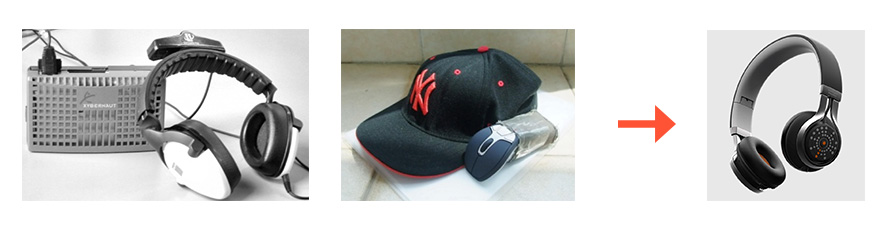
\includegraphics[width=\textwidth,height=\textheight,keepaspectratio]{./Figures/headset-development.jpg}
		\rule{35em}{0.5pt}
	\caption[Headset Development]{Wearable interfaces used before (left \cite{brewster_multimodaleyes-freeinteraction_2003} and middle \cite{park_gaze-directed_2011}) compaired with todays accessible interface (right \cite{gn_store_nord_intelligent_2013}).}
	\label{fig:headsets}
\end{figure}

With this interface it is possible to detect not only the head rotation (gyroscope) but also the acceleration (accelerometer) when the head is moving. There exists advanced algorithms for recognizing motion gestures \cite{lu_head_2005, kratz_combining_2013, akl_accelerometer-based_2010} but this project will use a simple Dynamic Time Warping algorithm \cite{meinard_muller_information_2007} as the gestures used are short and simple e.g. nodding or shaking the head and the focus is not on optimizing and precisioning the gestures.

\subsection{Audio as output modality}
Replacing visual with audio output has shown to have a positive effect when interacting in motion. Brewster showed, by compairing visual and audio feedback when pushing buttons on the same GUI, that it was difficult for users to devote all their visual attention to an interface while walking, running og driving and that the interaction workload decreased with audio feedback \cite{brewster_overcoming_2002}.

% Speech vs Non-speech audio
Audio output can in general be divided in two ways \cite{rocchesso_sounding_2003}:
\begin{description}
\item{1: \textit{Speech audio}}, can use a computer recorded human voice like in a guided audio tour for tourists.
\item{2: \textit{Non-speech audio}}, can be used for presenting more complex information e.g. music or other sounds.
\end{description}

Work has shown that non-speech audio is effective in improving the interaction in mobile environments \cite{pirhonen_gestural_2002, sawhney_nomadic_2000}.


% Maybe selective-attention and divided-attention defs.

\section{Spatial Audio Interface}

\subsection{Spatial Audio}

% From Brewster article (vazquez-alvarez_eyes-free_2011)
%Different attention demands impose different amounts of cognitive load on the user. When David is listening to the voicemail left by Stephen, he is focusing attention on the voicemail audio stream while monitoring his music (a se- lective-attention task). However, when David is talking to Stephen while interacting with his calendar using an audio menu to find a suitable time for their meeting, David is di- viding his attention between both audio streams (a divided- attention task). The first task results in less cognitive load, and the second in higher cognitive load.

% Spatial Sound (HRTF)
%HRTF: Good reference for 3d sound \cite{begault_3dd_1994}

% Audio menus

% Intelligent Headset



% OLD STUFF
% ---------
% motivation for audio and spatial sound feedback
%William W. Gaver, a pioneer in audio interfaces, has explored several aspects of using sound in interfaces including the intuitiveness of presenting complex information to users in the form of audio \cite{gaver_sonicfinder:_1989}. Similarly Graham explores the advantages in reaction time when using ”auditory icons” \cite{graham_use_1999}. In \cite{gaver_auditory_1986} Gaver presents the use of spatial sound icons. In doing so, he draws forward the unutilized potential of creating natural interaction through spatial audio.


\section{Related systems}
[TODO: intro]

% closely related to my project
Brewster et al. showed that novel interaction techniques based on sound and gesture can significantly improve the usability of a wearable device in particular under "eyes-free" mobile conditions and that head gestures was a successful interaction technique with egocentric sounds the most effective \cite{brewster_multimodaleyes-freeinteraction_2003}.

Park et al. also experimented, using head gesture input and aural output, with 1D and 2D menu interfaces \cite{park_gaze-directed_2011}.

Kajastila and Lokki has done a user study comparing auditory and visual menus controlled by the same free-hand gestures where the majority of the participants felt that an auditory circular menu was faster than a visual based menu \cite{kajastila_interaction_2013}.

\subsection{Systems properties overview}
[TODO]

Table compairing properties of related work (and this project) example fig. \ref{tab:related} (NOTE: temp, i need some input for this...).

\begin{table}[h] 
\caption{Related works properties comparison} % title name of the table 
%\centering % centering table

% Properties
% - In-motion interaction
% - Output modality
% - Input modality (Head, foot, hand)
% - Menu depth (1D, 2D)
% - Using accessible hardware
% - Controlling music application
% - 1-1 evaluation against real world application

\begin{tabular}{L{4cm}C{2cm}C{2cm}C{2cm}C{2cm}} \toprule
    Related work & Head gesture interaction & Spatial sound feedback & Music application & Accessible hardware \\ \midrule
    Multimodal eyes-free interaction techniques for wearable devices \cite{brewster_multimodaleyes-freeinteraction_2003}  & + & + & - & - \\ \midrule
    This project  & + & + & + & + \\ \bottomrule
\end{tabular}

\label{tab:related} 
\end{table}


\section{Summary}
[TODO]







